\documentclass{include/protokollclass}
% Main File - Based on protokollclass.cls
% Comments are mostly in English (and some in German, concerning the Praktikum)
% ------------------------------------------------------------------------------
% Further files in folder:
%  - include/cmds.tex (for macros and additional commands)
%  - include/kitlogo.pdf (for titlepage)
%  - lit.bib (bibtex bibliography database)
%  - include/titlepage.tex (for layout of titelpage)
% ------------------------------------------------------------------------------
% Useful Supplied Packages:
% amsmath, amssymb, mathtools, bbm, upgreek, nicefrac,
% siunitx, varioref, booktabs, graphicx, tikz, multicol





%% ---------------------------------------------
%% |    Informationen über dieses Protokoll    |
%% ---------------------------------------------
\newcommand{\praktikum}{P2}                % P1 oder P2
\newcommand{\semester}{SS17}            % z.B. "WS14/15" oder "SS15"

\newcommand{\wochentag}{Mo}                % Mo, Di, Mi oder Do
\newcommand{\gruppennr}{22}                % Zweistellige Gruppennummer

\newcommand{\nachnamea}{Becker}             % Nachname des ersten Praktikanten
\newcommand{\vornamea}{Alexander}               % Vorname des ersten Praktikanten
\newcommand{\nachnameb}{Voigtlaender}              % Nachname des zweiten Praktikanten
\newcommand{\vornameb}{Tim}              % Vorname des zweiten Praktikanten

\newcommand{\emailadressen}{uxehi@student.kit.edu, uoefa@student.kit.edu}
% optionale Angabe von Emailadresse(n) für den Kontakt mit dem Betreuer

\newcommand{\versuch}{Franck Hertz Versuch} % Name des Versuchs
\newcommand{\versuchsnr}{52}               % bitte die korrekte Nummer dem
                                           % Arbeitsplatz am Versuchstag
                                           % entnehmen
\newcommand{\fehlerrechnung}{Nein}         % Ob Fehlerrechnung im Versuch
                                           % durchgeführt wurde oder nicht

					   \newcommand{\betreuer}{Tim Storbeck / Julia Handl}      % Name des zuständigen Betreuers
\newcommand{\durchgefuehrt}{10.07.17}      % Datum, an dem der Versuch
                                           % durchgeführt wurde





%% --------------------------------------
%% |    Settings for Word Separation    |
%% --------------------------------------
% Help for separation:
% In German package the following hints are additionally available:
% "- = Additional separation
% "| = Suppress ligation and possible separation (e.g. Schaf"|fell)
% "~ = Hyphenation without separation (e.g. bergauf und "~ab)
% "= = Hyphenation with separation before and after
% "" = Separation without a hyphenation (e.g. und/""oder)

% Describe separation hints here:
\hyphenation
{
    über-nom-me-nen an-ge-ge-be-nen
    %Pro-to-koll-in-stan-zen
    %Ma-na-ge-ment  Netz-werk-ele-men-ten
    %Netz-werk Netz-werk-re-ser-vie-rung
    %Netz-werk-adap-ter Fein-ju-stier-ung
    %Da-ten-strom-spe-zi-fi-ka-tion Pa-ket-rumpf
    %Kon-troll-in-stanz
}





% um die Titelseite per PDF-reader auszufüllen. Vorgefertigte Daten
% können in Datei 'data.tex' modifiziert werden.
%\setboolean{forminput}{true}
% um die Anmerkungen zu den Textfeldern anzeigen zu lassen
%\setboolean{showannotations}{true}
% Erneuern der Seitenzahl in jedem Kapitel
%\setboolean{chapResetPageNumb}{true}
% Einbinden der Kapitelnummer in der Seitenzahl
%\setboolean{chapWiseNumb}{true}
% english or ngerman (new german für neue deutsche Rechtschreibung statt german)
\SelectLanguage{ngerman}
\usepackage{pdfpages}




%% -----------------------
%% |    Main Document    |
%% -----------------------
\begin{document}
% Titlepage und ToC
\FrontMatter

% coordinates for background border
\newcommand{\diameter}{20}
\newcommand{\xone}{-15}
\newcommand{\xtwo}{160}
\newcommand{\yone}{15}
\newcommand{\ytwo}{-253}

\newcommand{\hoehea}{60}
\newcommand{\hoeheb}{60}




\begin{titlepage}
    % background border
    \begin{tikzpicture}[overlay]
    \draw[color=gray]  
            (\xone mm, \yone mm)
      -- (\xtwo mm, \yone mm)
    arc (90:0:\diameter pt) 
      -- (\xtwo mm + \diameter pt , \ytwo mm) 
        -- (\xone mm + \diameter pt , \ytwo mm)
    arc (270:180:\diameter pt)
        -- (\xone mm, \yone mm);
    \end{tikzpicture}
    
    % KIT logo
    \begin{textblock}{10}[0,0](4.5,2.5)
        
\includegraphics[width=.25\textwidth]{include/kitlogo.pdf}
    \end{textblock}
    \changefont{phv}{m}{n}    % helvetica
    \begin{textblock}{10}[0,0](5.5,2.2)
        \begin{flushright}
            \Large FAKULTÄT FÜR PHYSIK\\Praktikum Klassische Physik
        \end{flushright}
    \end{textblock}
    
    \begin{textblock}{10}[0,0](4.2,3.1)
        \begin{tikzpicture}[overlay]
        \draw[color=gray]
            (\xone mm + 5 mm, -12 mm)
         -- (\xtwo mm + \diameter pt - 5 mm, -12 mm);
        \end{tikzpicture}
    \end{textblock}
    
    \Large
    % Zeile 1
    \begin{textblock}{12}[0,0](3.58,4.4)
        \mytextfield{Prak.}{\praktikum}{0.9cm}{17pt}
                    {P1/P2}{2}{Praktikum}
    \end{textblock}
    \begin{textblock}{12}[0,0](5.53,4.4)
        \mytextfield{Semester}{\semester}{2.6cm}{17pt}
        {z.B. \glqq WS14/15\grqq\ oder \glqq SS15\grqq}{0}{Semester}
    \end{textblock}
    \begin{textblock}{12}[0,0](9.53,4.4)
        \mytextfield{Wochentag}{\wochentag}{1.3cm}{17pt}
                    {Mo/Di/Mi/Do}{2}{Wochentag}2
    \end{textblock}
    \begin{textblock}{12}[0,0](12.88,4.4)
       \mytextfield{Gruppennr.}{\gruppennr}{1.06cm}{17pt}
                   {\#\#}{2}{Gruppennummer}
    \end{textblock}
    
    % Zeile 2
    \begin{textblock}{12}[0,0](3.58,4.95)
        \mytextfield{Name}{\nachnamea}{6cm}{17pt}
                    {}{0}{Name1}
    \end{textblock}
    \begin{textblock}{12}[0,0](9.53,4.95)
        \mytextfield{Vorname}{\vornamea}{6cm}{17pt}
                    {}{0}{Vorname1}
    \end{textblock}
    
    % Zeile 3
    \begin{textblock}{12}[0,0](3.58,5.5)
        \mytextfield{Name}{\nachnameb}{6cm}{17pt}
                    {}{0}{Name2}
    \end{textblock}
    \begin{textblock}{12}[0,0](9.53,5.5)
        \mytextfield{Vorname}{\vornameb}{6cm}{17pt}
                    {}{0}{Vorname2}
    \end{textblock}
    
    % Zeile 4
    \begin{textblock}{12}[0,0](3.64,6.05)
       \normalsize\mytextfield{Emailadresse(n)}{\emailadressen}{13.1cm}{10pt}
                              {Optional}{0}{Emailadressen}
    \end{textblock}
    
    % Zeile 5
    \begin{textblock}{12}[0,0](3.58,7)
        \mytextfield{Versuch}{\versuch\ (\praktikum-\versuchsnr)}{9.45cm}{14pt}
                    {z.B. \glqq Galvanometer (P1-13)\grqq\ oder \glqq %
                     Mikrowellenoptik (P2-15)\grqq}{0}{Versuch}
    \end{textblock}
    \begin{textblock}{12}[0,0](12.58,7)
       \mytextfield{Fehlerrech.}{\fehlerrechnung}{1.46cm}{17pt}
                   {Ja/Nein}{4}{Fehlerrechnung}
    \end{textblock}
    
    % Zeile 6
    \begin{textblock}{12}[0,0](3.58,7.55)
        \mytextfield{Betreuer}{\betreuer}{7cm}{17pt}{}{0}{Betreuer}
    \end{textblock}
    \begin{textblock}{12}[0,0](10.82,7.55)
        \mytextfield{Durchgeführt am}{\durchgefuehrt}{2.53cm}{17pt}
                    {TT.MM.JJ}{8}{Durchfuehrung}
    \end{textblock}
    
    % Querstrich
    \begin{textblock}{20}[0,0](0,7.9)\tiny\centering
        Wird vom Betreuer ausgefüllt.
    \end{textblock}
    \begin{tikzpicture}[overlay]
    \draw[color=gray]
        (\xone mm + 5 mm, -95 mm)
     -- (\xtwo mm + \diameter pt - 5 mm, -95 mm);
    \end{tikzpicture}
    
    % Zeile 1
    \begin{textblock}{12}[0,0](3.65,8.57)
        \myTtextfield{1. Abgabe am}{}{2.5cm}{17pt}
                     {}
    \end{textblock}
    
    % Block 1
    \begin{tikzpicture}[overlay]
    \draw[color=gray]  
        (\xone mm + 10 mm, -107.5 mm)
     -- (\xtwo mm + \diameter pt - 10 mm, -107.5 mm)
     -- (\xtwo mm + \diameter pt - 10 mm, -107.5 mm - \hoehea mm)
     -- (\xone mm + 10 mm, -107.5 mm - \hoehea mm)
     -- (\xone mm + 10 mm, -107.5 mm);
    \end{tikzpicture}
    \begin{textblock}{20}[0,0](3.8,9.2)
        \myTtextfield{Rückgabe am}{}{2.5cm}{17pt}
                     {}
    \end{textblock}
    \begin{textblock}{20}[0,0](8.7,9.2)
        \smash{Begründung:}
    \end{textblock}
    
    % Zeile 2
    \begin{textblock}{12}[0,0](3.65,12.6)
        \myTtextfield{2. Abgabe am}{}{2.5cm}{17pt}
                     {}
    \end{textblock}
    
    % Block 2
    \begin{tikzpicture}[overlay]
    \draw[color=gray]  
        (\xone mm + 10 mm, -180 mm)
     -- (\xtwo mm + \diameter pt - 10 mm, -180 mm)
     -- (\xtwo mm + \diameter pt - 10 mm, -180 mm - \hoehea mm)
     -- (\xone mm + 10 mm, -180 mm - \hoehea mm)
     -- (\xone mm + 10 mm, -180 mm);
    \end{tikzpicture}
    \begin{textblock}{12}[0,0](4,13.25)
        \smash{Ergebnis:~~~~+~~~/~~~0~~~/~~~-}
    \end{textblock}
    \begin{textblock}{12}[0,0](9.5,13.25)
        \smash{Fehlerrechnung:~~~Ja~~~/~~~Nein}
    \end{textblock}
    \begin{textblock}{12}[0,0](3.8,13.72)
        \myTtextfield{Datum}{}{2.5cm}{17pt}
                     {}
    \end{textblock}
    \begin{textblock}{12}[0,0](8.3,13.72)
        \myTtextfield{Handzeichen}{}{5.5cm}{17pt}
                     {}
    \end{textblock}
    \begin{textblock}{12}[0,0](4,14.25)\Large
        \smash{Bemerkungen:}
    \end{textblock}
    
    
    
    % lowest text blocks concerning the KIT
    \begin{textblock}{10}[0,0](4,16.8)
        \tiny{KIT -- Universität des Landes Baden-Württemberg und nationales %
              Forschungszentrum in der Helmholtz-Gemeinschaft}
    \end{textblock}
    \begin{textblock}{10}[0,0](14,16.75)
        \large{\textbf{www.kit.edu}}
    \end{textblock}
\end{titlepage}
 %\cleardoublepage

\begingroup \let\clearpage\relax    % in order to avoid listoffigures and
\tableofcontents                    % listoftables on new pages
\listoffigures
\listoftables
\endgroup
%\cleardoublepage



% Contents
\MainMatter
\chapter{Aufgabe1: Messung der Frank Hertz Kurve unter verschiedenen Bedingungen}
In diesem Versuch nutzen wir eine Quecksilber-Franck-Hertz-Röhre um verschiedene Effekte zu untersuchen.
\begin{figure}
	\centering
	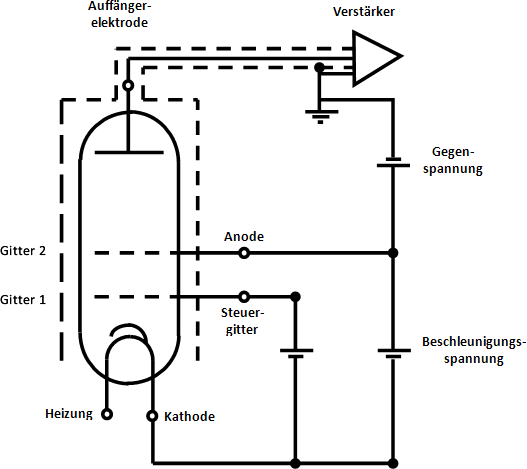
\includegraphics[width=0.5\textwidth]{../Daten/Aufgabe1/Aufbau.png}
	\caption{Skizze einer Franck-Hertz-Röhre \cite{FHR}}
\end{figure}
\section{Aufbau}
Bei der Franck-Hertz-Röhre handelt es sich um einen abgeschlossenen, mit Gas gefüllten Glaskörper. In diesem werden mithilfe einer Heizspirale freie Elektronen erzeugt, die dann mithilfe einer angelegten Spannung und eines Steuergitters beschleunigt werden. Auf der gegenüberliegenden Seite der Röhre befindet sich eine Auffangelektrode. Zwischen den beiden befindet sich ein Gitter, welches als Anode zur Heizspirale agiert. Zwischen Gitter und Auffangelektrode befindet sich ein schwaches Gegenfeld. Bei unserer Messung erwarten wir, dass wir mit steigender Beschleunigungsspannung eine zunehmende Anzahl von Elektronen bei der Auffangelektrode registrieren, wobei es allerdings in gleichbleibenden Abständen Abfälle gibt. Diese Form wird auch Franck-Herz-Kurve genannt. Um den Versuch durchzuführen bauten wir ihn zunächst wie in der Aufgabenstellung beschrieben auf.
\section{Bestimmung der Kontaktspannung zwischen Kathode und Anode}
Dann ermitteln wir die Thermokontaktspannung. Bei der Aufnahme der Daten haben wir leider Versäumt den Graphen der Messung bei 120$\; ^\circ $C abzuspeichern, weswegen für diesen nur die Daten ohne Bild vorliegen.
\begin{figure}
	\centering
	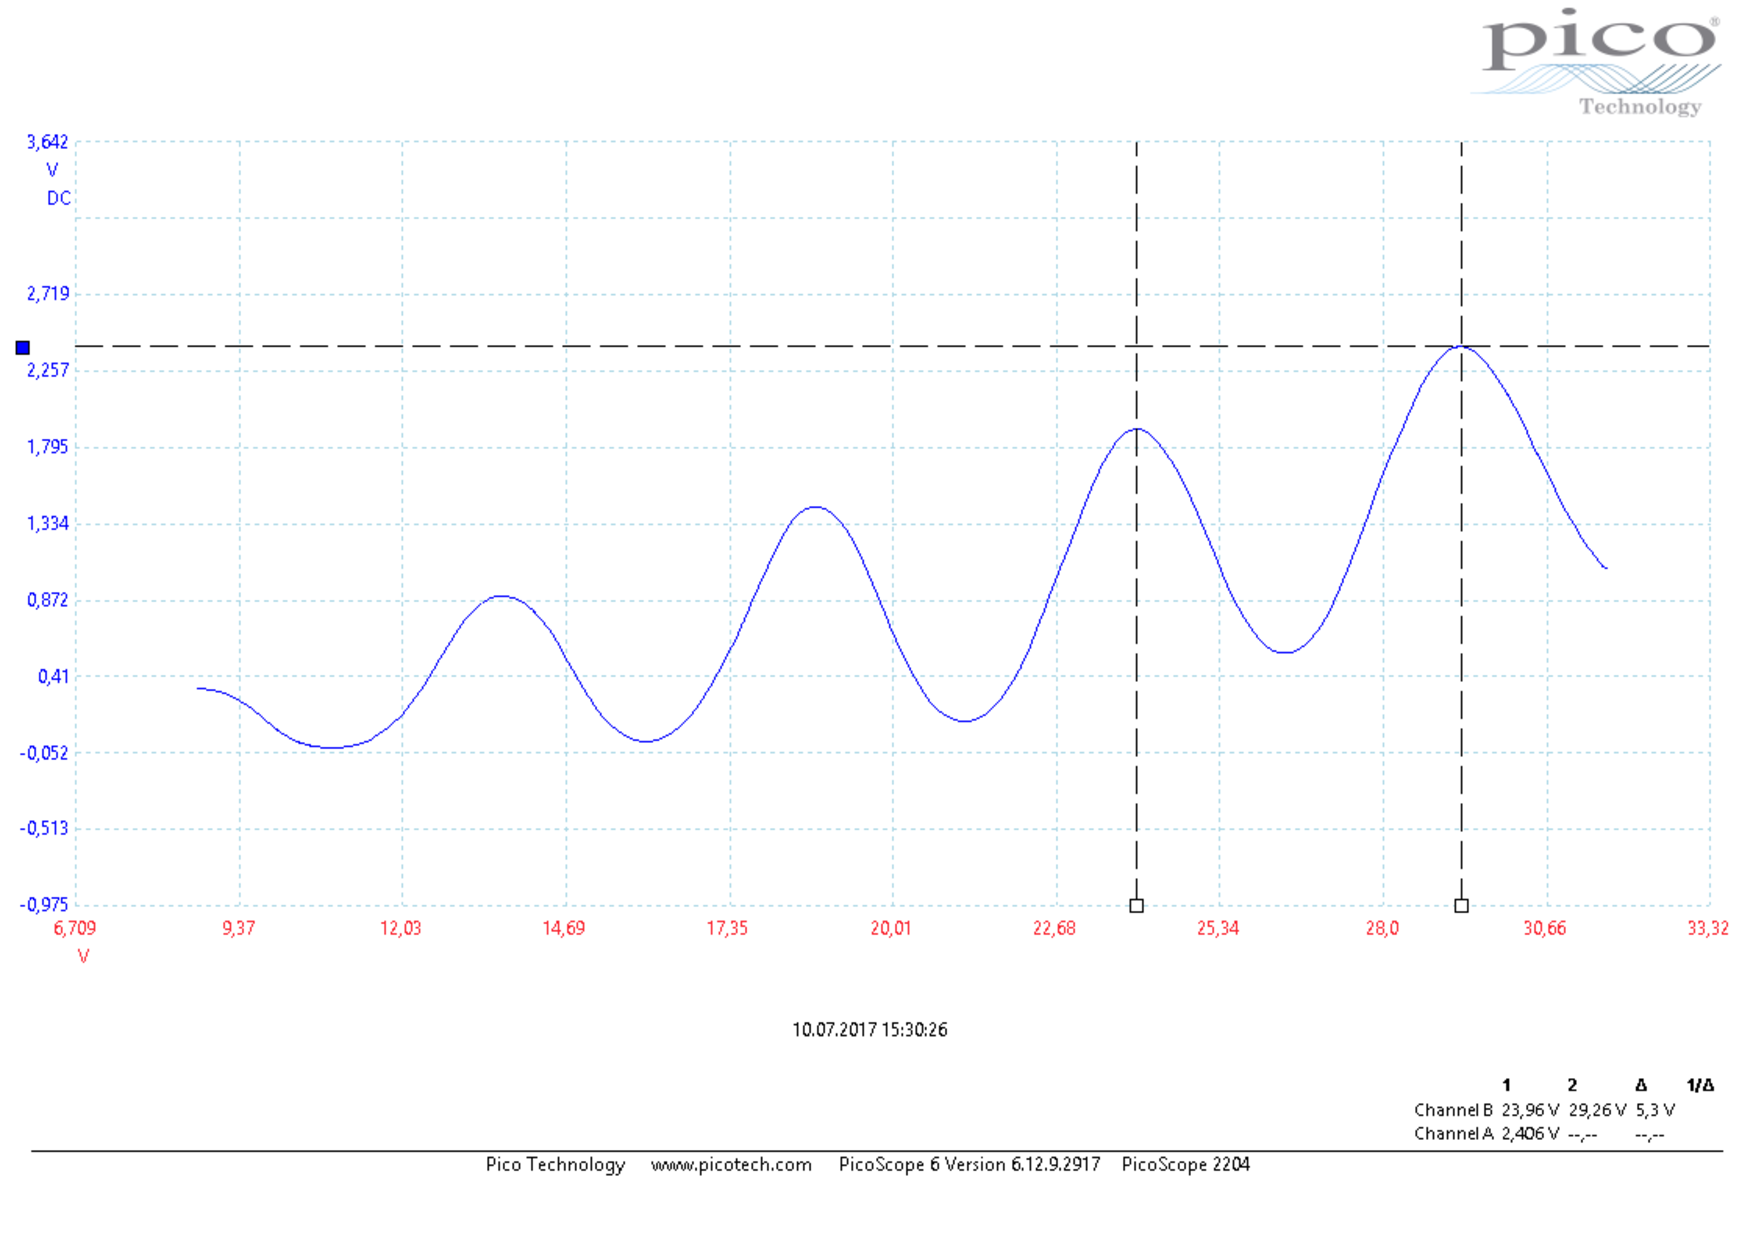
\includegraphics[width=\textwidth]{../Daten/Aufgabe1/Frank_Hertz_140.pdf}
	\caption{Franck-Herz-Kurve bei 140$ ^\circ $C}
	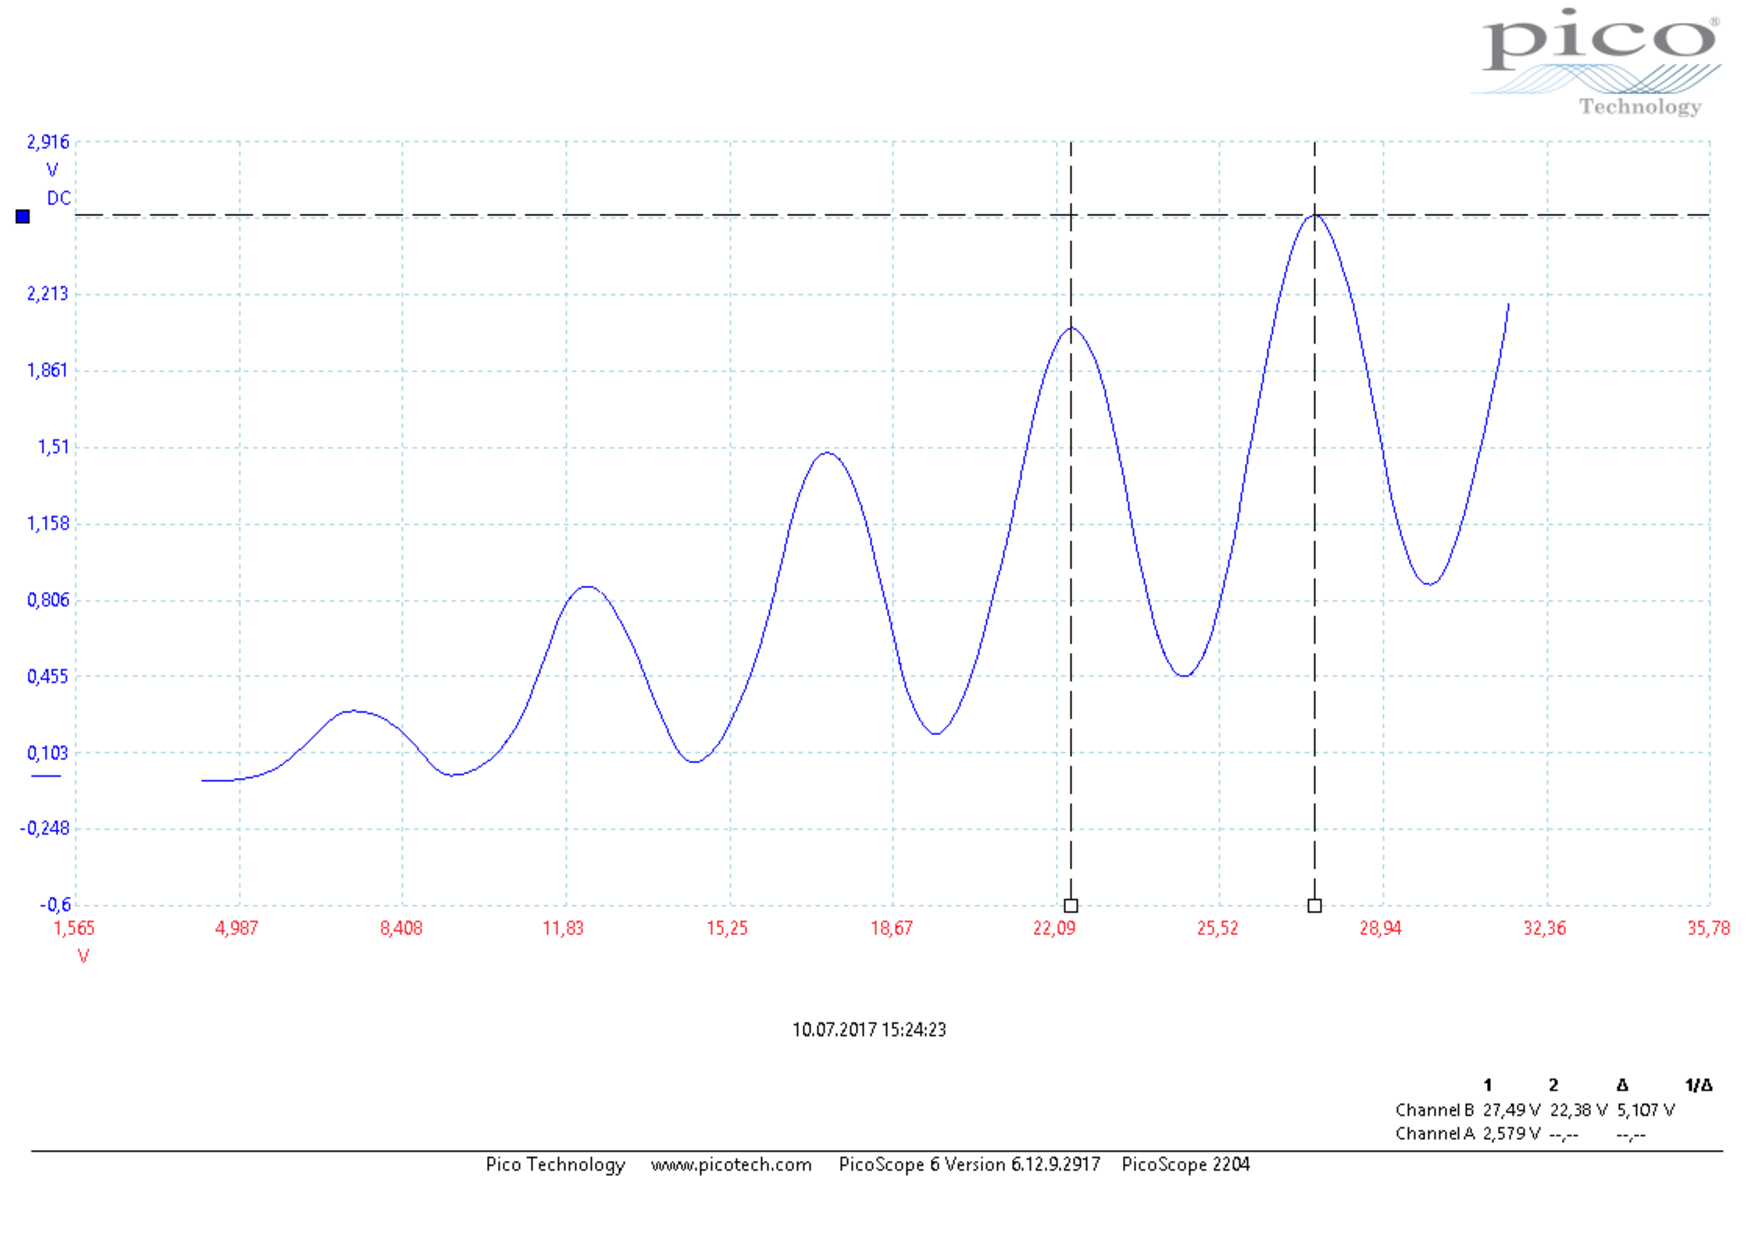
\includegraphics[width=\textwidth]{../Daten/Aufgabe1/Frank_Hertz_150.pdf}
	\caption{Franck-Herz-Kurve bei 150$ ^\circ $C}
\end{figure}
\begin{figure}
	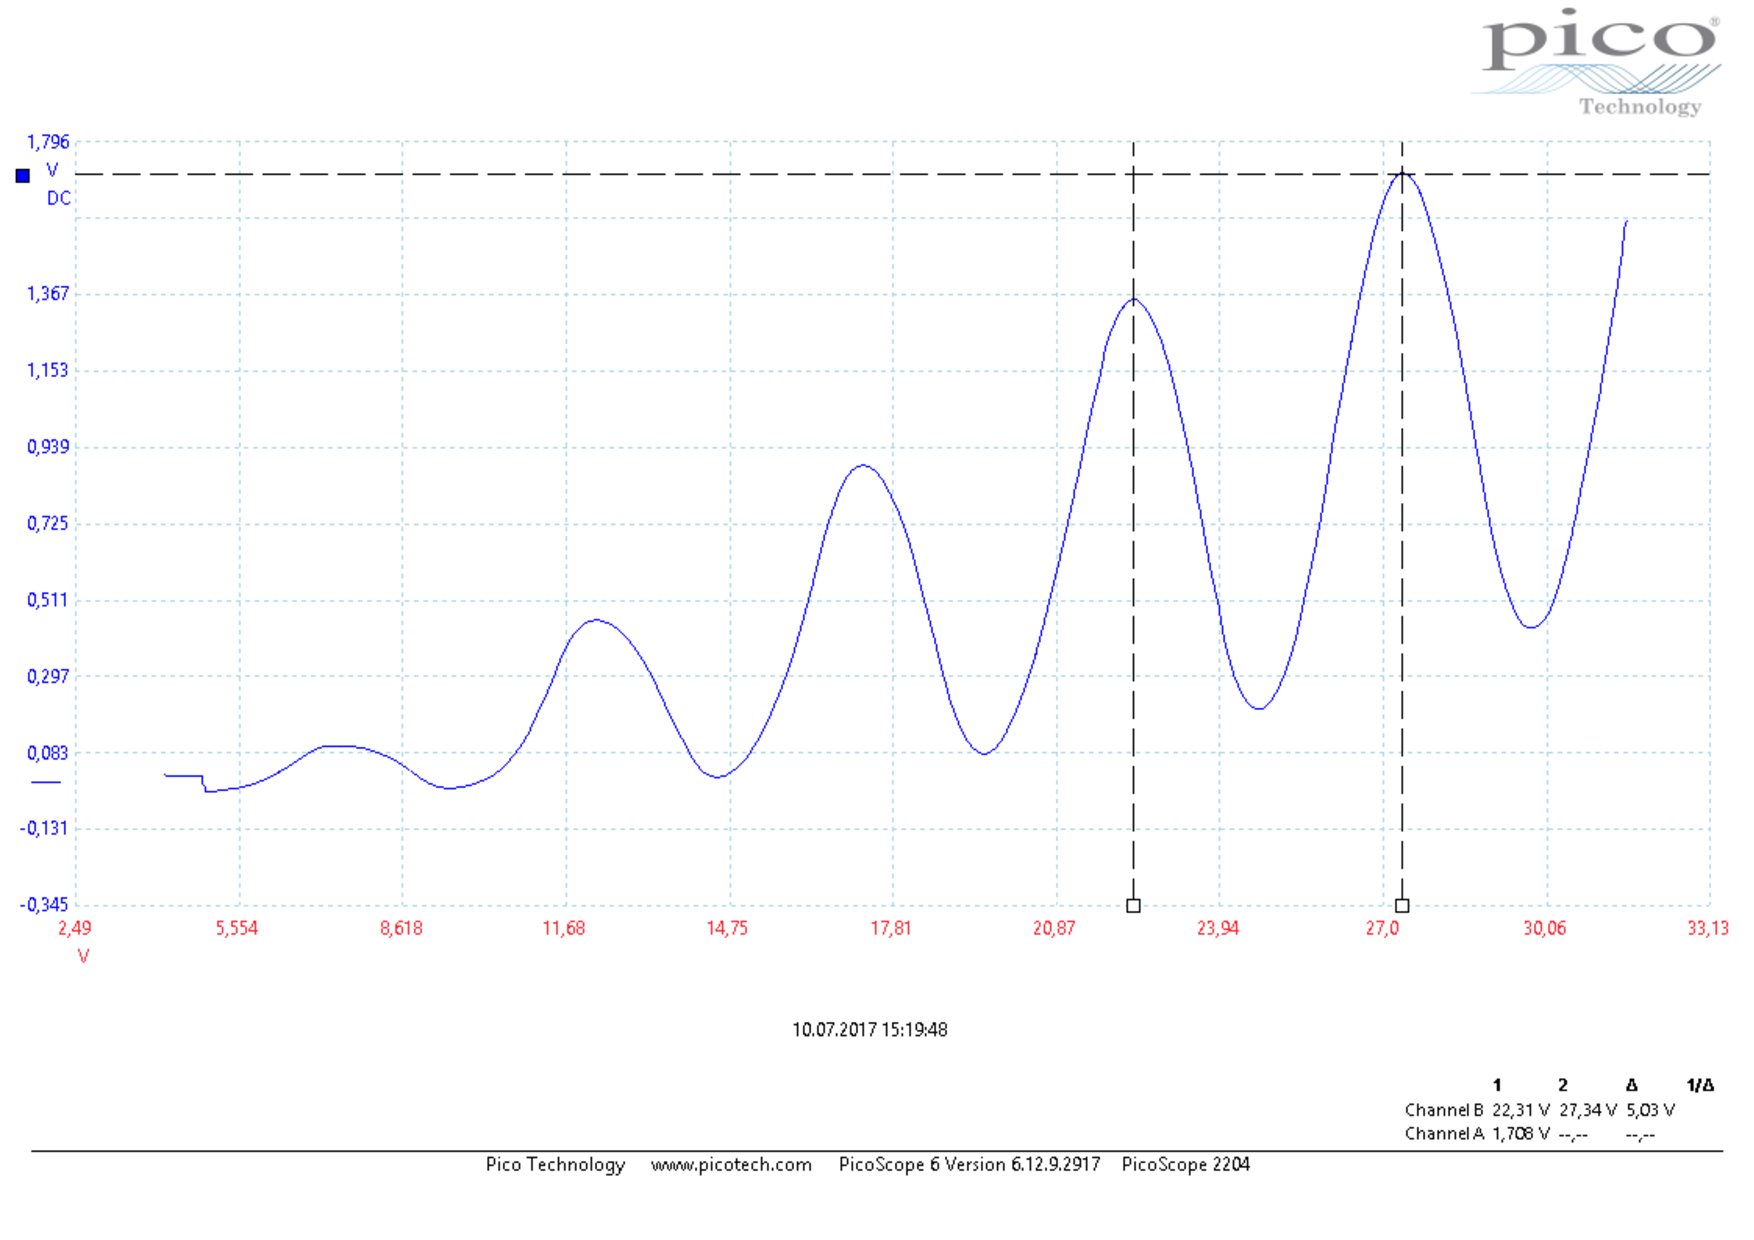
\includegraphics[width=\textwidth]{../Daten/Aufgabe1/Frank_Hertz_160.pdf}
	\caption{Franck-Herz-Kurve bei 160$ ^\circ $C}
	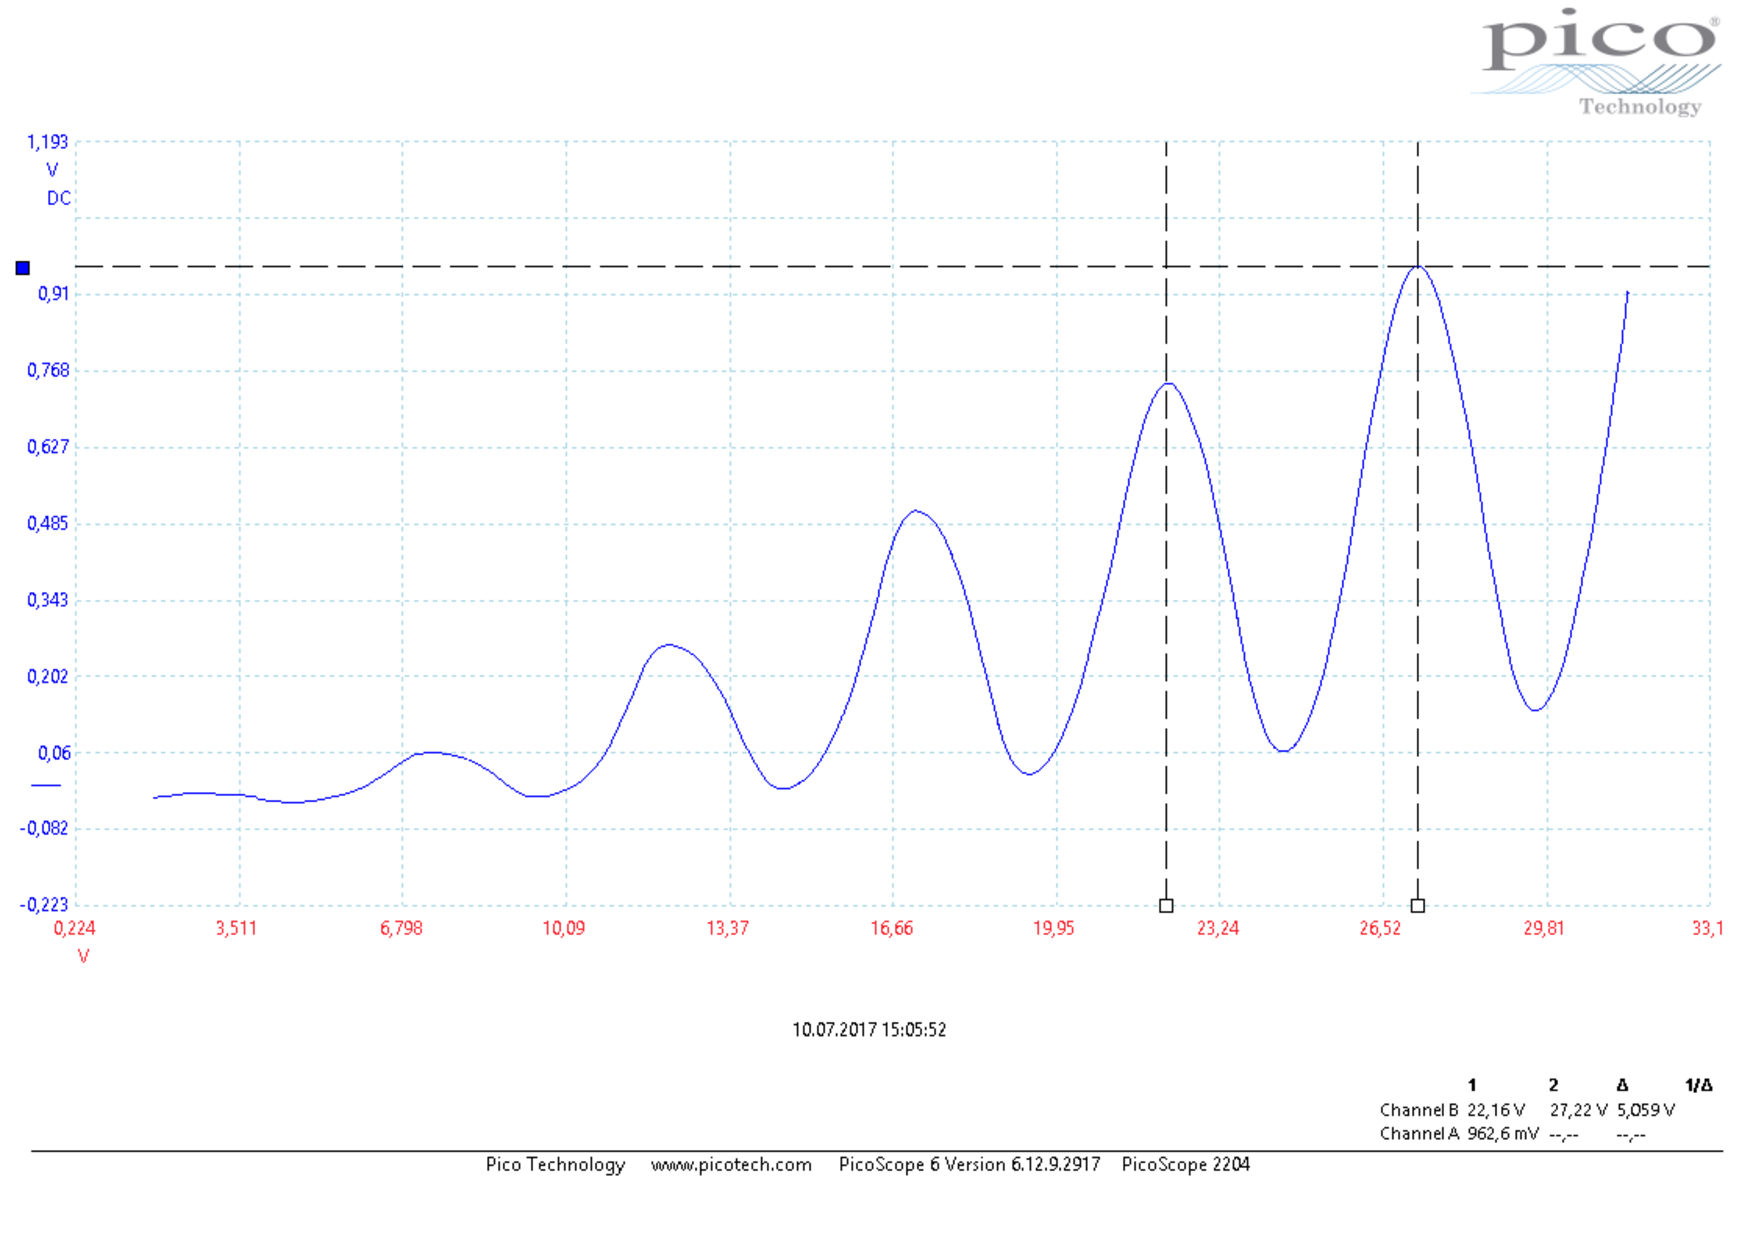
\includegraphics[width=\textwidth]{../Daten/Aufgabe1/Frank_Hertz_170.pdf}
	\caption{Franck-Herz-Kurve bei 170$ ^\circ $C}
\end{figure}
Somit erhalten wir die jeweiligen Thermospannungen über die Formel
\begin{align*}
U_{Th}=U_{n}+U_{1}-n\cdot \overline{\Delta U}\text{,}
\end{align*}
Hierbei ist $ \overline{\Delta U} $ der gemittelte Wert der $ \Delta U $ und $ U_{n} $ die Spannung des n-ten Peaks.

Aus diesen Werten erhalten wir nun den gemittelten Wert $ \overline{U_{th}} =6,407\; $V.
\begin{table}
	\centering
	\caption {Thermospannung in Abhängigkeit der Temperatur}
	\begin{tabular}{|c|c|}
		\hline
		Temperatur in $^\circ$C & U$_{th}$ in V \\ \hline
		170           &     6,379     \\ \hline
		160           &     6,381     \\ \hline
		150           &     6,294     \\ \hline
		140           &     6,553     \\ \hline
		120           &     6,427     \\ \hline
	\end{tabular} 
\end{table}
\section{Das Raumladungsgesetz}
Nun überprüfen wir das Raumladungsgesetz bei einer Temperatur von 120 $ ^\circ $C. Wir erwarten einen Zusammenhang der Form $I\propto U_{2}^{3/2}  $, weswegen wir die Messdaten wie folgt fitten
\begin{align*}
\log(I)=a\cdot \log(U_{2})+b\text{.}
\end{align*}
\begin{figure}
	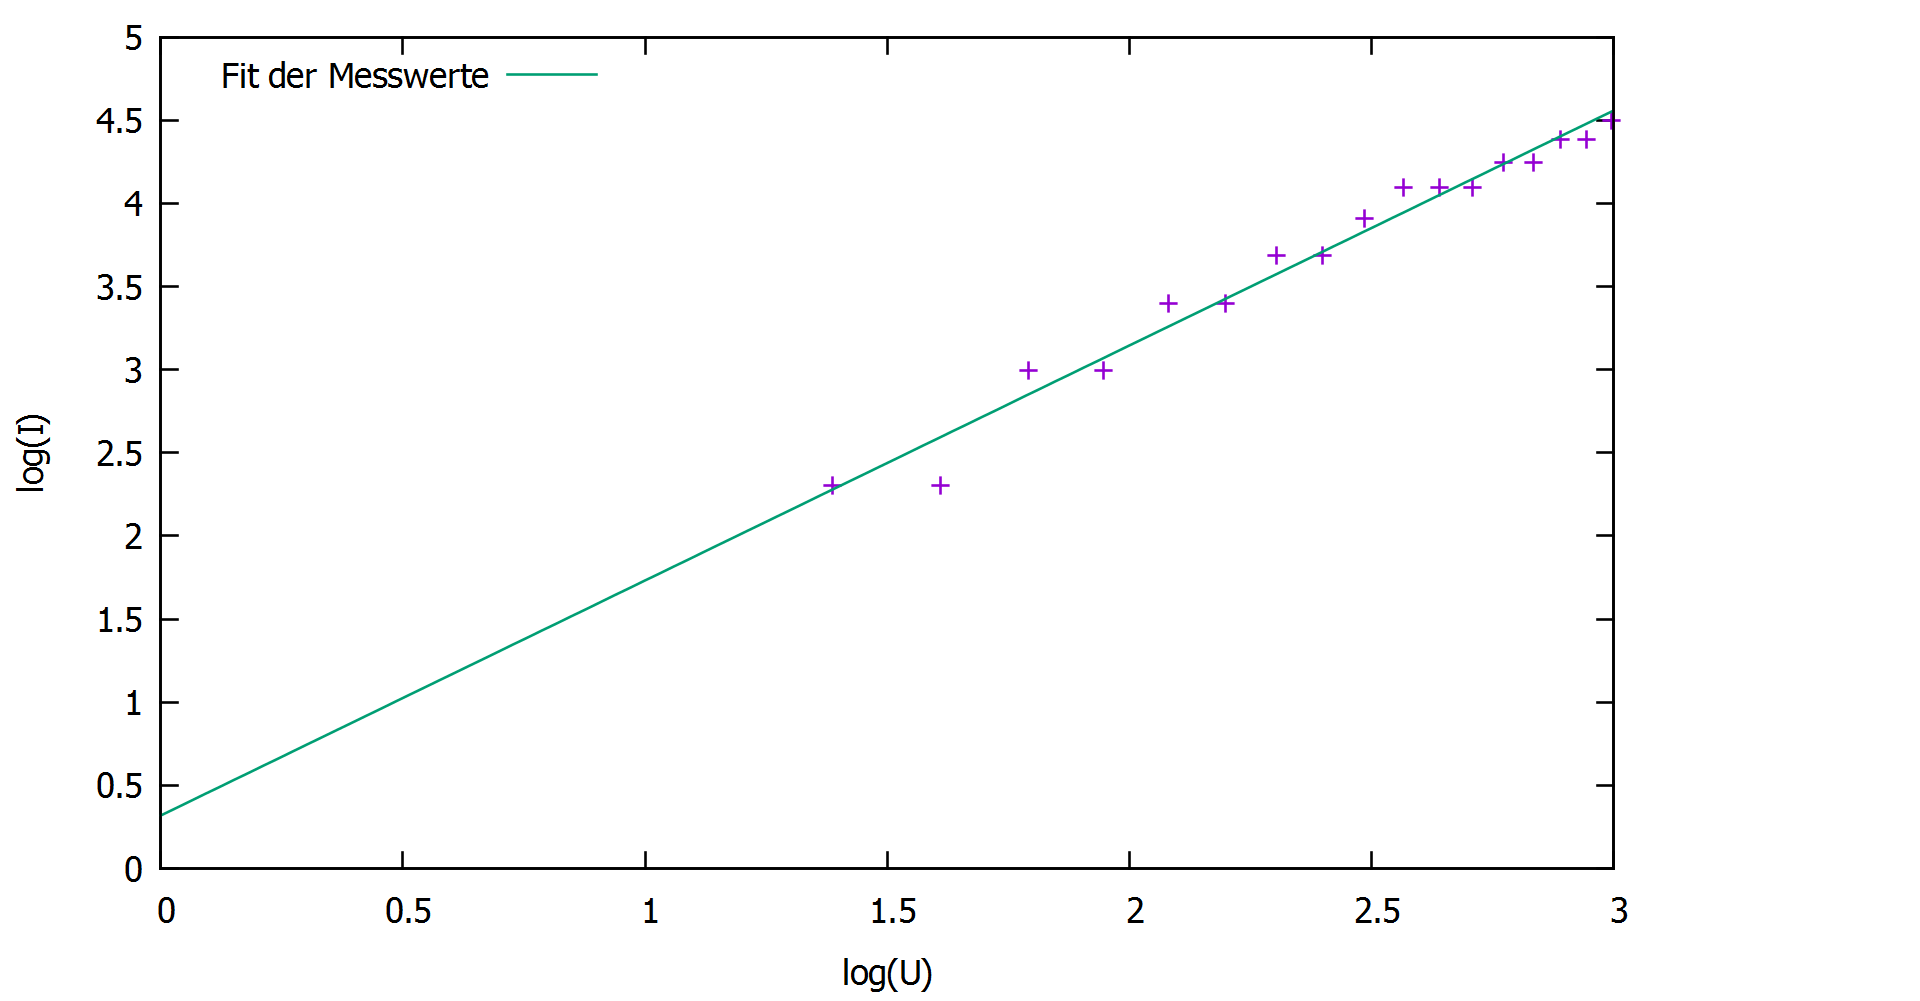
\includegraphics[width=\textwidth]{../Daten/Aufgabe1/Aufgabe1_3.png}
	\caption{Lineare Regression zu Kapitel 1.3 in Form von log(I)=a$ \cdot $log(U$ _2 $)+b}
\end{figure}
Die mit Gnuplot erstellte Funktion hat die Steigung a=1,414. Vergleicht man dies mit dem erhofften Wert(1,5) erhält man einen Fehler von 5,7\%.

\section{Ionisationsarbeit}
Nun wollen wir die Ionisationsarbeit von Quecksilber bei 120 $ ^\circ $C bestimmen.
\subsection{Bestimmung durch Graphische Ermittelung des Anstiegspunkts}
Zunächst bestimmen wir die Ionisationsarbeit indem wir die Stromstärke I$ _{in} $ über die Spannung U$ _2 $ auftragen und zwei Geraden durch die Messpunkte legen. Der Schnittpunkt der Geraden beschreibt dann den Anstiegspunkt und damit die Ionisationsarbeit. Hierbei stellt sich jedoch heraus, das einige Werte zu stark von der Form einer Geraden abweichen, weswegen diese Messpunkte vernachlässigt wurden. 
\begin{figure}
	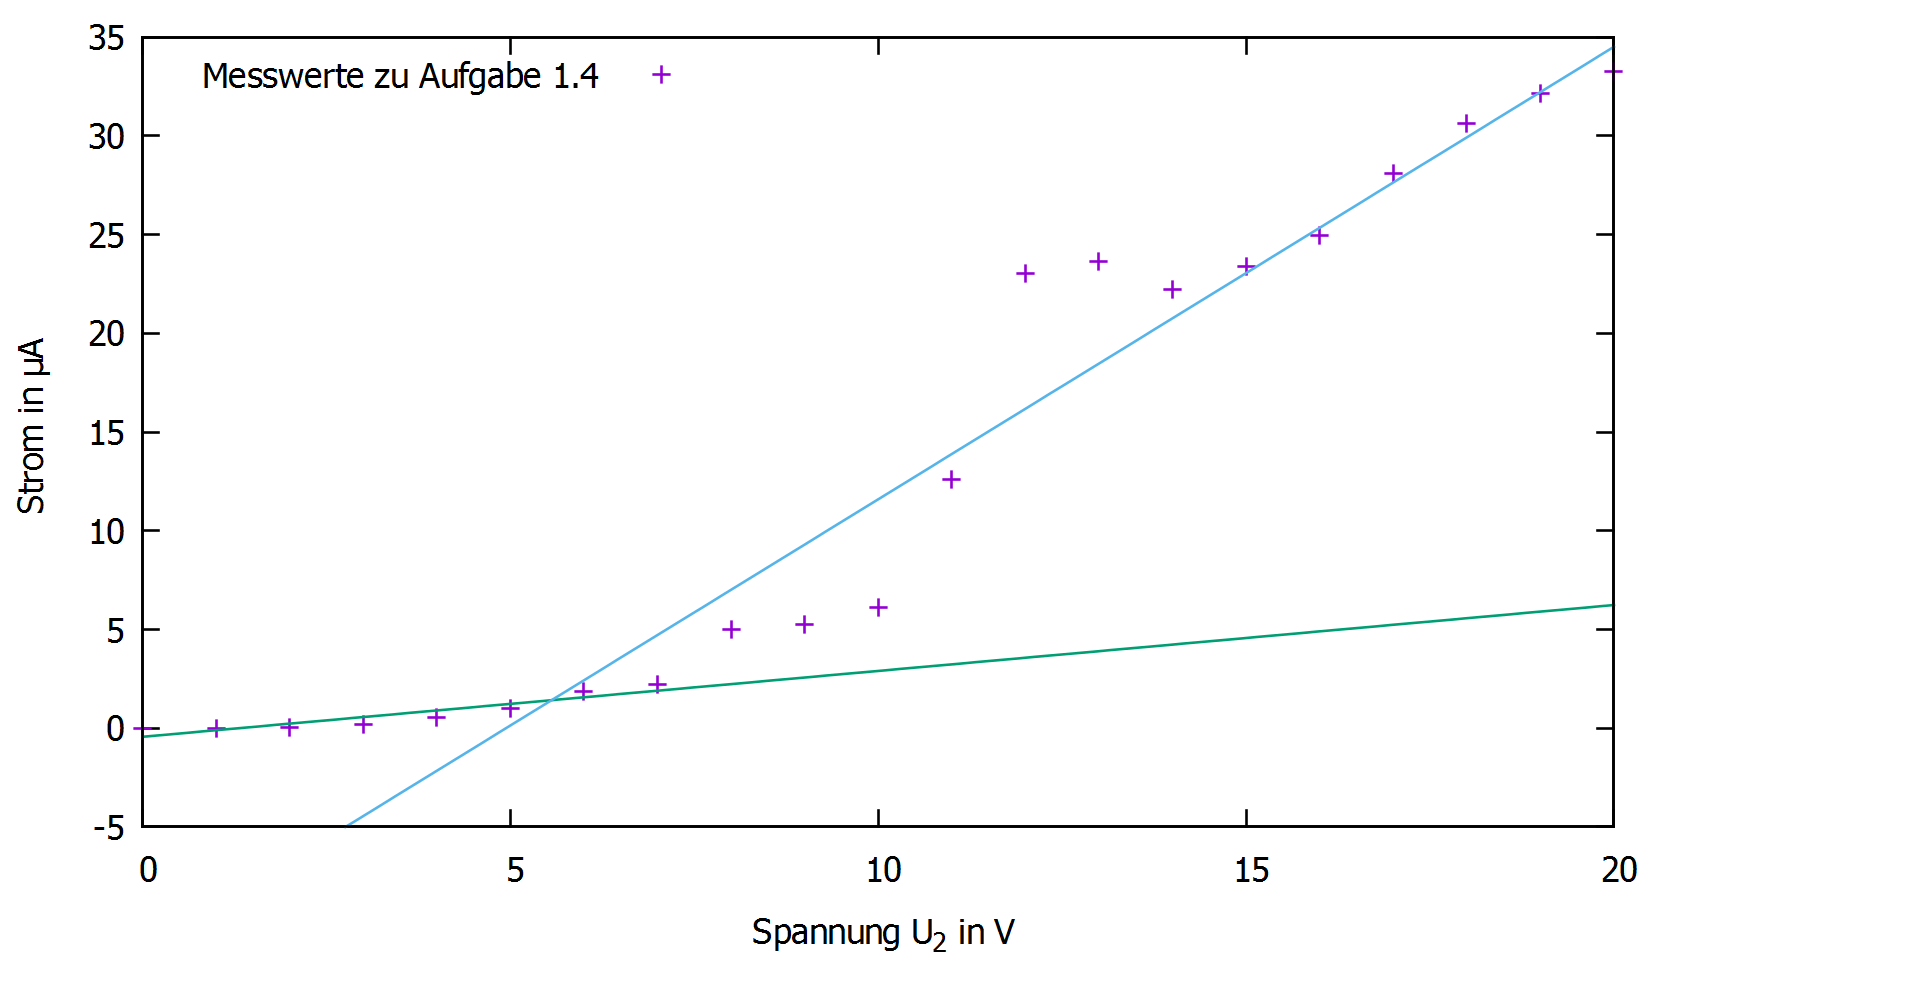
\includegraphics[width=\textwidth]{../Daten/Aufgabe1/Aufgabe1_4.png}
	\caption{Fit der Messwerte zu Aufgabe 1.4.1}
\end{figure}

Der Schnittpunkt befindet sich bei U$ _2 $= 5,579 V. Verrechnen wir nun noch die Thermokontaktspannung aus Kapitel 1.1 erhalten wir die Ionisationsarbeit 11,986 eV. Dies entspricht einer Abweichung vom Literaturwert (10,44 eV) von 12,9\%. Wir vermuten, dass dieser Fehler aufgrund von nicht beachteten Umständen während der Versuchsdurchführung entstand, da die gemessenen Werte ebenfalls sehr ungewöhnlich aussehen.
\subsection{Bestimmung über Auffängerspannung}
\begin{figure}
	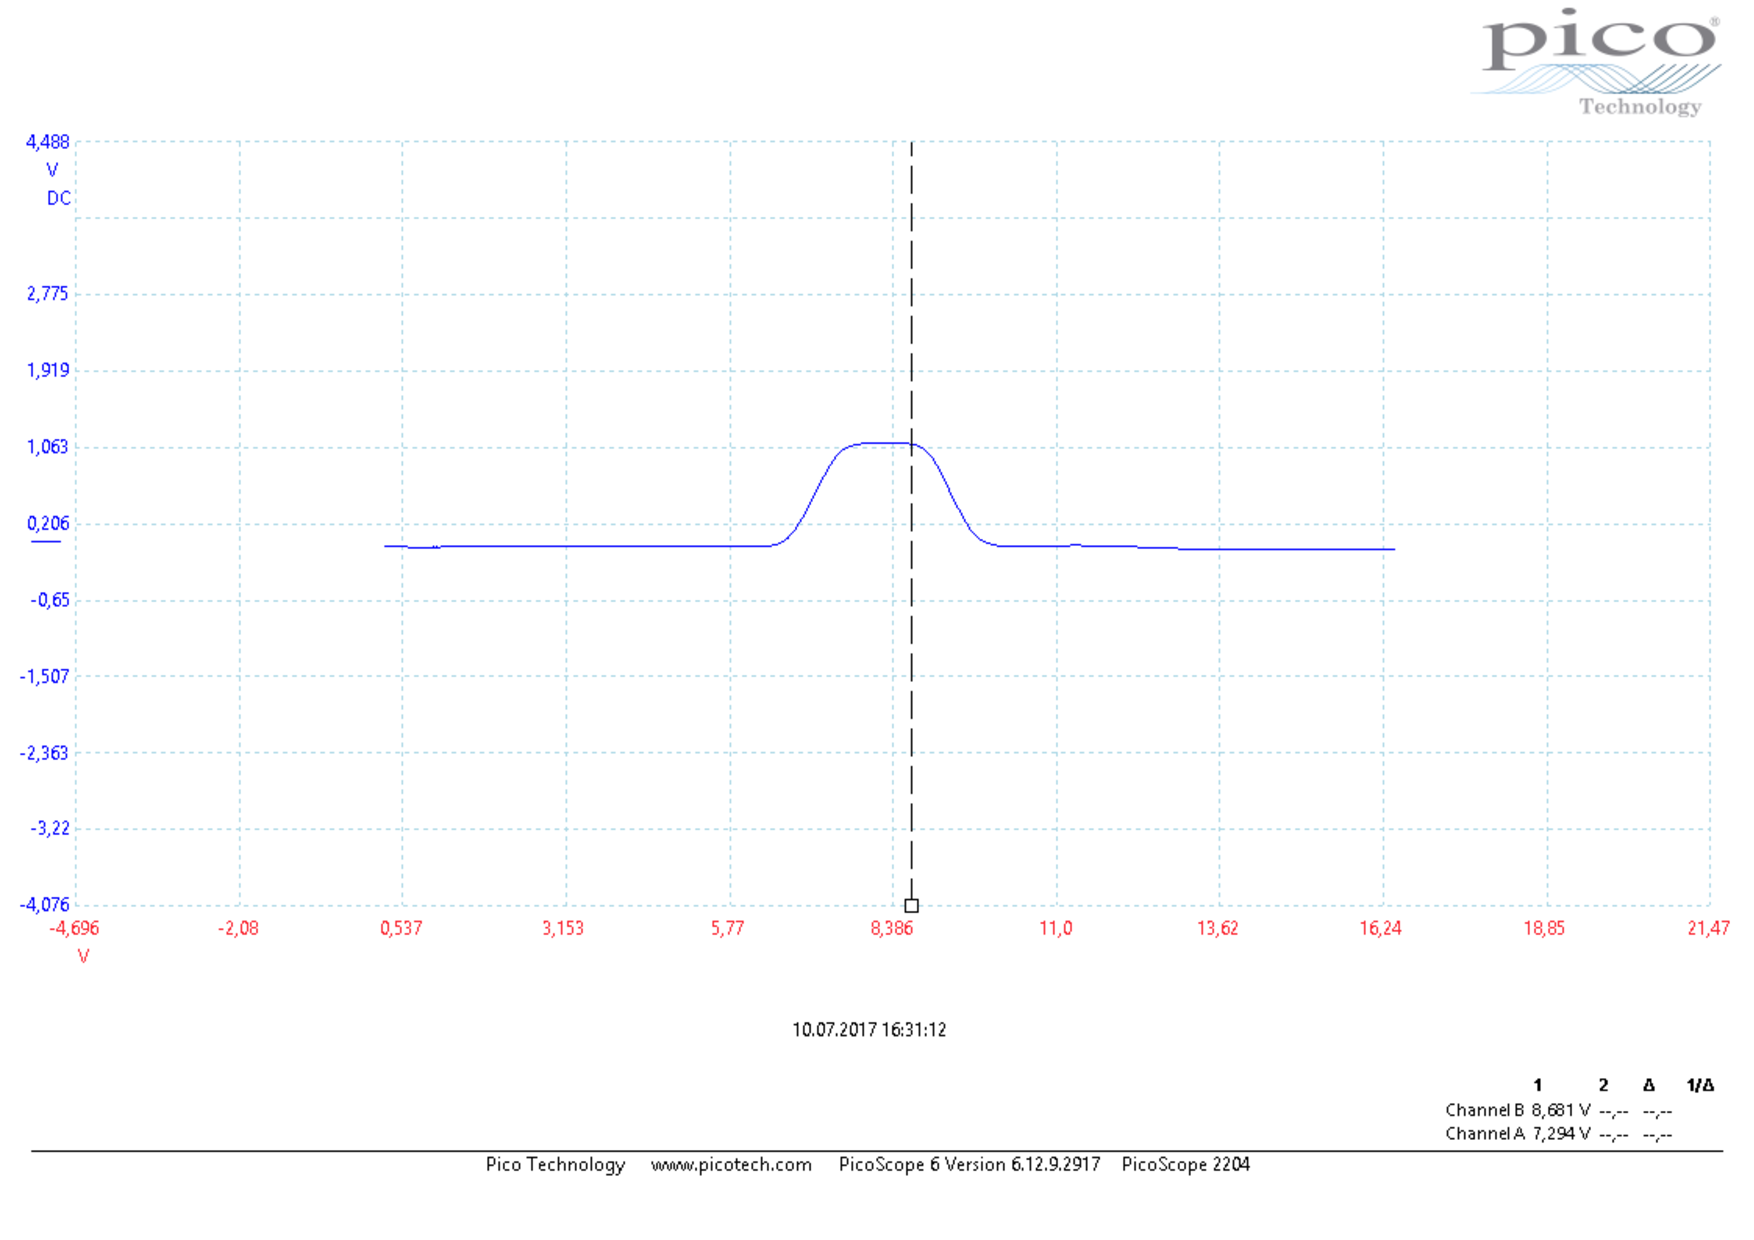
\includegraphics[width=\textwidth]{../Daten/Aufgabe1/Frank_Hertz_1_4_b_2.pdf}
	\caption{Auffängerspannung über Beschleunigungsspannung zu Aufgabe 1.4.2}
\end{figure}
Als zweite Variante wurde die Spannung direkt aus der im Graphen ablesbaren Auffängerspannung ermittelt, wobei dieser ebenfalls Ungewöhnlich aussieht. Mit dieser Methode erhalten wir eine Ionisationsarbeit von 10,789 eV, was einem Fehler von 3,2\% entspricht.
\section{Emissionsspektrum der Gasentladung}
Als letztes betrachten wir die Gasentladung mithilfe eines Taschenspektroskops. Hierbei konnten wir die Farben Rot, Gelb, Grün und Lila erkennen. Es ist möglich, dass es noch weitere sichtbare Farben gab, die wegen angelassenem Raumlicht nicht erkennbar waren.
 %\cleardoublepage
\chapter{Aufgabe 2: Bestimmung der Frank Hertz Kurve fuer die Zweite Anregung}
In dieser Aufgabe berechnen wir die Aktivität des Cs Präparates.
Hierbei gilt die Formel:
\begin{align*}
A=\dfrac{N-N_{grund}}{(1-p_{tot})\cdot p_{nw}}
\end{align*}
Wobei $ N_{grund}=8242 $ die Anzahl an Messwerten ist, die durch das Untergrundspektrum hinzukommt.
\begin{center}
	Tabelle 1: Messwerte zu Aufgabe 2
\end{center}
\begin{center}
	\begin{tabular}{c|c|c|c|c}
		Abstand in cm & Totzeit $p_{tot}$ in \% & Nachweisw. $p_{nw}$ in \% & Messwerte N & Aktivität in Bq \\ \hline
		1       &          24,24          &            5,0            &   995460    &      86872      \\
		3       &           8,9           &            1,2            &   353885    &     105392      \\
		6       &           3,4           &            0,4            &   143751    &     116899
	\end{tabular} 
\end{center}

Man würde hierbei erwarten, dass die Aktivitäten unabhängig vom Abstand konstant bleiben. Dies ist hier nicht der Fall, da scheinbar ein weiterer Abstands-abhängiger Faktor hinzukommt. Wir halten es für wahrscheinlich, dass die Tabelle zur Nachweiswahrscheinlichkeit nicht optimal auf den Versuch abgestimmt ist, weswegen der Abstand ungewollter weise einen Einfluss auf die Aktivität hat.
\chapter{Aufgabe 3: Der Franck Hertz versuch mit Neon}
\section{Versuchsaufbau}
In diesem Versuchsteil wird nun effektiv der gleiche Versuch wie in Kapitel 1 durchgeführt, mit dem entscheidenden Unterschied, dass anstelle des verwendeten Quecksilbers nun Neon zum Einsatz kommt.
Da ein anderes Gas verwendet wird, werden auch andere Anregungsenergien erwartet.
Bei der Anregung von Neon durch Elektronen ist ein Übergang von Grundzustand in einen der 10 3p Zustände am wahrscheinlichsten. Diese Liegen in einem Bereich von 18,4 - 19 V \cite{HND1}.
Beim Übergang vom 3p in den 3s Zustand werden Photonen im sichtbaren teil des Spektrums emittiert. Der Übergang aus dem 3s Zustand in den Grundzustand emittiert Photonen im UV-Bereich.
\subsection{Heizen des Versuchsaufbaus}
Heizen des Versuchsaufbaus ergibt hier wenig Sinn, da nun ein Gas anstelle eines Dampfes vorliegt. Damit ändert sich die Teilchendichte nicht mit der Temperatur.
\section{Beobachtungen und Interpretation}
Die in \ref{tab:gemesseneAnregungsenergieNeon} gelisteten, gemessenen Maxima bestätigen die geäusserten Vermutungen.
Im Stoßraum können zudem pro gemessenen Peak eine leuchtende Scheibe gesehen werden. Diese Scheiben sind die Stoßzonen der verschiedenen Elektronen.
\begin{table}
	\centering
	\caption{Anregungsniveaus von Neon}
	\begin{tabular}{c c}
		Anzahl der Stöße & Gegenspannung des Peaks in V \\
		\midrule
		1 & 18,3 \\
		2 & 25,6 \\
		3 & 55,7 \\
	\end{tabular}
	\label{tab:gemesseneAnregungsenergieNeon}
\end{table}
Eine Lineare Regression der gemessenen Werte ergibt eine Steigung von 18,7 V / Anregung was in dem von der Vorbereitungsliteratur angegebenen Intervall liegt.


%\chapter{Aufgabe 4: Statistische Analyse des Untergrundspektrums}
%\input{./chap/chapter4.tex}

% appendix for more or less interesting calculations
%\Appendix
%\chapter{\appendixname} \addcontentsline{toc}{chapter}{\appendixname}
% to make the appendix appear in ToC without number. \appendixname =
% Appendix or Anhang (depending on chosen language)
%\section{Erster Abschnitt des Anhangs}
Dies ist der erste ganz tolle Abschnitt des Anhangs. %\cleardoublepage


% Bibliography
\TheBibliography

%\BIBTEX
%use if you want citations to appear even if they are not referenced to:
%\nocite{*} or maybe \nocite{Kon64,And59} for specific entries
%\nocite{*}
\bibliographystyle{babalpha}
\bibliography{lit.bib}

% THEBIBLIOGRAPHY
%\begin{thebibliography}{000}
%    \bibitem{ident}Entry into Bibliography.
%\end{thebibliography}
\end{document}
